\begin{center}


	\tikzset{every picture/.style={line width=0.75pt}} %set default line width to 0.75pt        

	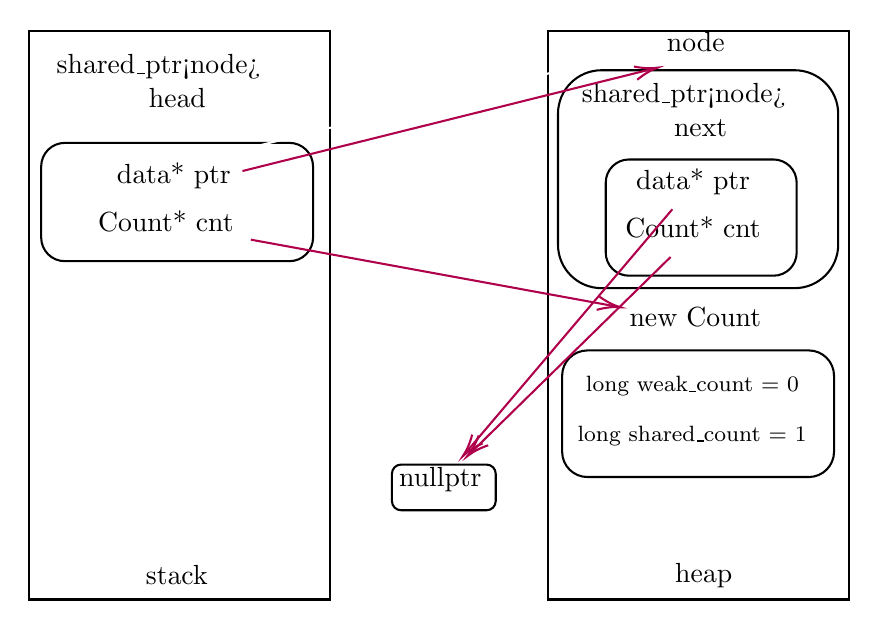
\begin{tikzpicture}[x=0.75pt,y=0.75pt,yscale=-1,xscale=1]
	%uncomment if require: \path (0,300); %set diagram left start at 0, and has height of 300
	
	%Rounded Rect [id:dp2187423114764504] 
	\draw   (139,77.4) .. controls (139,71.1) and (144.1,66) .. (150.4,66) -- (258.6,66) .. controls (264.9,66) and (270,71.1) .. (270,77.4) -- (270,111.6) .. controls (270,117.9) and (264.9,123) .. (258.6,123) -- (150.4,123) .. controls (144.1,123) and (139,117.9) .. (139,111.6) -- cycle ;
	%Shape: Rectangle [id:dp2941975065261839] 
	\draw   (133,12) -- (278,12) -- (278,286) -- (133,286) -- cycle ;
	%Shape: Rectangle [id:dp09704288189667065] 
	\draw   (383,12) -- (528,12) -- (528,286) -- (383,286) -- cycle ;
	%Rounded Rect [id:dp5478085044935208] 
	\draw   (388,52) .. controls (388,40.4) and (397.4,31) .. (409,31) -- (502,31) .. controls (513.6,31) and (523,40.4) .. (523,52) -- (523,115) .. controls (523,126.6) and (513.6,136) .. (502,136) -- (409,136) .. controls (397.4,136) and (388,126.6) .. (388,115) -- cycle ;
	%Rounded Rect [id:dp12609398185570142] 
	\draw   (411,85.2) .. controls (411,79.01) and (416.01,74) .. (422.2,74) -- (491.8,74) .. controls (497.99,74) and (503,79.01) .. (503,85.2) -- (503,118.8) .. controls (503,124.99) and (497.99,130) .. (491.8,130) -- (422.2,130) .. controls (416.01,130) and (411,124.99) .. (411,118.8) -- cycle ;
	%Rounded Rect [id:dp20297270277383261] 
	\draw   (390,178.2) .. controls (390,171.46) and (395.46,166) .. (402.2,166) -- (508.8,166) .. controls (515.54,166) and (521,171.46) .. (521,178.2) -- (521,214.8) .. controls (521,221.54) and (515.54,227) .. (508.8,227) -- (402.2,227) .. controls (395.46,227) and (390,221.54) .. (390,214.8) -- cycle ;
	%Rounded Rect [id:dp060261680865621337] 
	\draw   (308,225.4) .. controls (308,222.97) and (309.97,221) .. (312.4,221) -- (353.6,221) .. controls (356.03,221) and (358,222.97) .. (358,225.4) -- (358,238.6) .. controls (358,241.03) and (356.03,243) .. (353.6,243) -- (312.4,243) .. controls (309.97,243) and (308,241.03) .. (308,238.6) -- cycle ;
	
	% Text Node
	\draw (145,22) node [anchor=north west][inner sep=0.75pt]   [align=left] {shared\_ptr<node>\\ \ \ \ \ \ \ \ \ \ \ head};
	% Text Node
	\draw (439,11) node [anchor=north west][inner sep=0.75pt]   [align=left] {node};
	% Text Node
	\draw (174,74) node [anchor=north west][inner sep=0.75pt]   [align=left] {data* ptr};
	% Text Node
	\draw (165,97) node [anchor=north west][inner sep=0.75pt]   [align=left] {Count* cnt};
	% Text Node
	\draw (188,268) node [anchor=north west][inner sep=0.75pt]   [align=left] {stack};
	% Text Node
	\draw (443,267) node [anchor=north west][inner sep=0.75pt]   [align=left] {heap};
	% Text Node
	\draw (398,36) node [anchor=north west][inner sep=0.75pt]   [align=left] {shared\_ptr<node>\\ \ \ \ \ \ \ \ \ \ \ next};
	% Text Node
	\draw (424.2,77) node [anchor=north west][inner sep=0.75pt]   [align=left] {data* ptr};
	% Text Node
	\draw (419,100) node [anchor=north west][inner sep=0.75pt]   [align=left] {Count* cnt};
	% Text Node
	\draw (421,144) node [anchor=north west][inner sep=0.75pt]   [align=left] {new Count};
	% Text Node
	\draw (400,177) node [anchor=north west][inner sep=0.75pt]  [font=\footnotesize] [align=left] {long weak\_count = 0};
	% Text Node
	\draw (396,201) node [anchor=north west][inner sep=0.75pt]  [font=\footnotesize] [align=left] {long shared\_count = 1};
	% Text Node
	\draw (310,221) node [anchor=north west][inner sep=0.75pt]   [align=left] {nullptr};
	% Connection
	\draw [color={rgb, 255:red, 255; green, 255; blue, 255 }  ,draw opacity=1 ]   (233.01,70) -- (434.06,19.94) ;
	\draw [shift={(436,19.45)}, rotate = 166.02] [color={rgb, 255:red, 255; green, 255; blue, 255 }  ,draw opacity=1 ][line width=0.75]    (10.93,-3.29) .. controls (6.95,-1.4) and (3.31,-0.3) .. (0,0) .. controls (3.31,0.3) and (6.95,1.4) .. (10.93,3.29)   ;
	% Connection
	\draw [color={rgb, 255:red, 175; green, 0; blue, 75 }  ,draw opacity=1 ]   (236,79.56) -- (434.06,30.24) ;
	\draw [shift={(436,29.76)}, rotate = 166.02] [color={rgb, 255:red, 175; green, 0; blue, 75 }  ,draw opacity=1 ][line width=0.75]    (10.93,-3.29) .. controls (6.95,-1.4) and (3.31,-0.3) .. (0,0) .. controls (3.31,0.3) and (6.95,1.4) .. (10.93,3.29)   ;
	% Connection
	\draw [color={rgb, 255:red, 175; green, 0; blue, 75 }  ,draw opacity=1 ]   (240,112.63) -- (416.03,144.83) ;
	\draw [shift={(418,145.18)}, rotate = 190.36] [color={rgb, 255:red, 175; green, 0; blue, 75 }  ,draw opacity=1 ][line width=0.75]    (10.93,-3.29) .. controls (6.95,-1.4) and (3.31,-0.3) .. (0,0) .. controls (3.31,0.3) and (6.95,1.4) .. (10.93,3.29)   ;
	% Connection
	\draw [color={rgb, 255:red, 175; green, 0; blue, 75 }  ,draw opacity=1 ]   (443.09,98) -- (343.4,215.48) ;
	\draw [shift={(342.11,217)}, rotate = 310.32] [color={rgb, 255:red, 175; green, 0; blue, 75 }  ,draw opacity=1 ][line width=0.75]    (10.93,-3.29) .. controls (6.95,-1.4) and (3.31,-0.3) .. (0,0) .. controls (3.31,0.3) and (6.95,1.4) .. (10.93,3.29)   ;
	% Connection
	\draw [color={rgb, 255:red, 175; green, 0; blue, 75 }  ,draw opacity=1 ]   (442.24,121) -- (345.69,215.6) ;
	\draw [shift={(344.26,217)}, rotate = 315.59] [color={rgb, 255:red, 175; green, 0; blue, 75 }  ,draw opacity=1 ][line width=0.75]    (10.93,-3.29) .. controls (6.95,-1.4) and (3.31,-0.3) .. (0,0) .. controls (3.31,0.3) and (6.95,1.4) .. (10.93,3.29)   ;
	
	\end{tikzpicture}
	
{\tt (1)}
\end{center}